\documentclass[a4paper,12pt]{article}

\usepackage{amsmath}
\usepackage{graphicx}
\usepackage{hyperref}
\usepackage{geometry}

\geometry{top=2.5cm, bottom=2.5cm, left=2.5cm, right=2.5cm}

\title{Projekt Egzaminacyjny}
\author{Oliwia Wądołowska}
\date{\today}

\begin{document}

\maketitle

\begin{abstract}
Projekt przedstawia analizę log-zwrotów kursów akcji spółki Celon Pharma SA, przeprowadzoną na podstawie danych z dnia 1 stycznia 2022 roku do 31 grudnia 2023 roku. Celem pracy jest analiza zmian w kursach akcji oraz testowanie hipotezy o równych rozkładach log-zwrotów przy użyciu rozkładów normalnego i t-Studenta.
\end{abstract}

\tableofcontents
\newpage

\section{Wstęp}
Wybór spółki: Celon Pharma SA jest jednym z liderów w branży ABC, produkuje i sprzedaje produkty XYZ, posiadające silną pozycję na rynku krajowym i międzynarodowym. Akcje tej spółki są notowane na warszawskiej giełdzie, a ich analiza pozwala na zrozumienie dynamiki zmian cen akcji na rynku.

\section{Analiza Log-Zwrotów Spółki XYZ}
\subsection{Wykresy Kursów Zamknięcia i Log-Zwrotów}
Na poniższym wykresie przedstawiono zmiany w kursach zamknięcia akcji Spółki XYZ na przestrzeni roku 2022, jak również wykres log-zwrotów, które opisują dzienne zmiany wartości akcji.

\begin{figure}[h!]
\centering
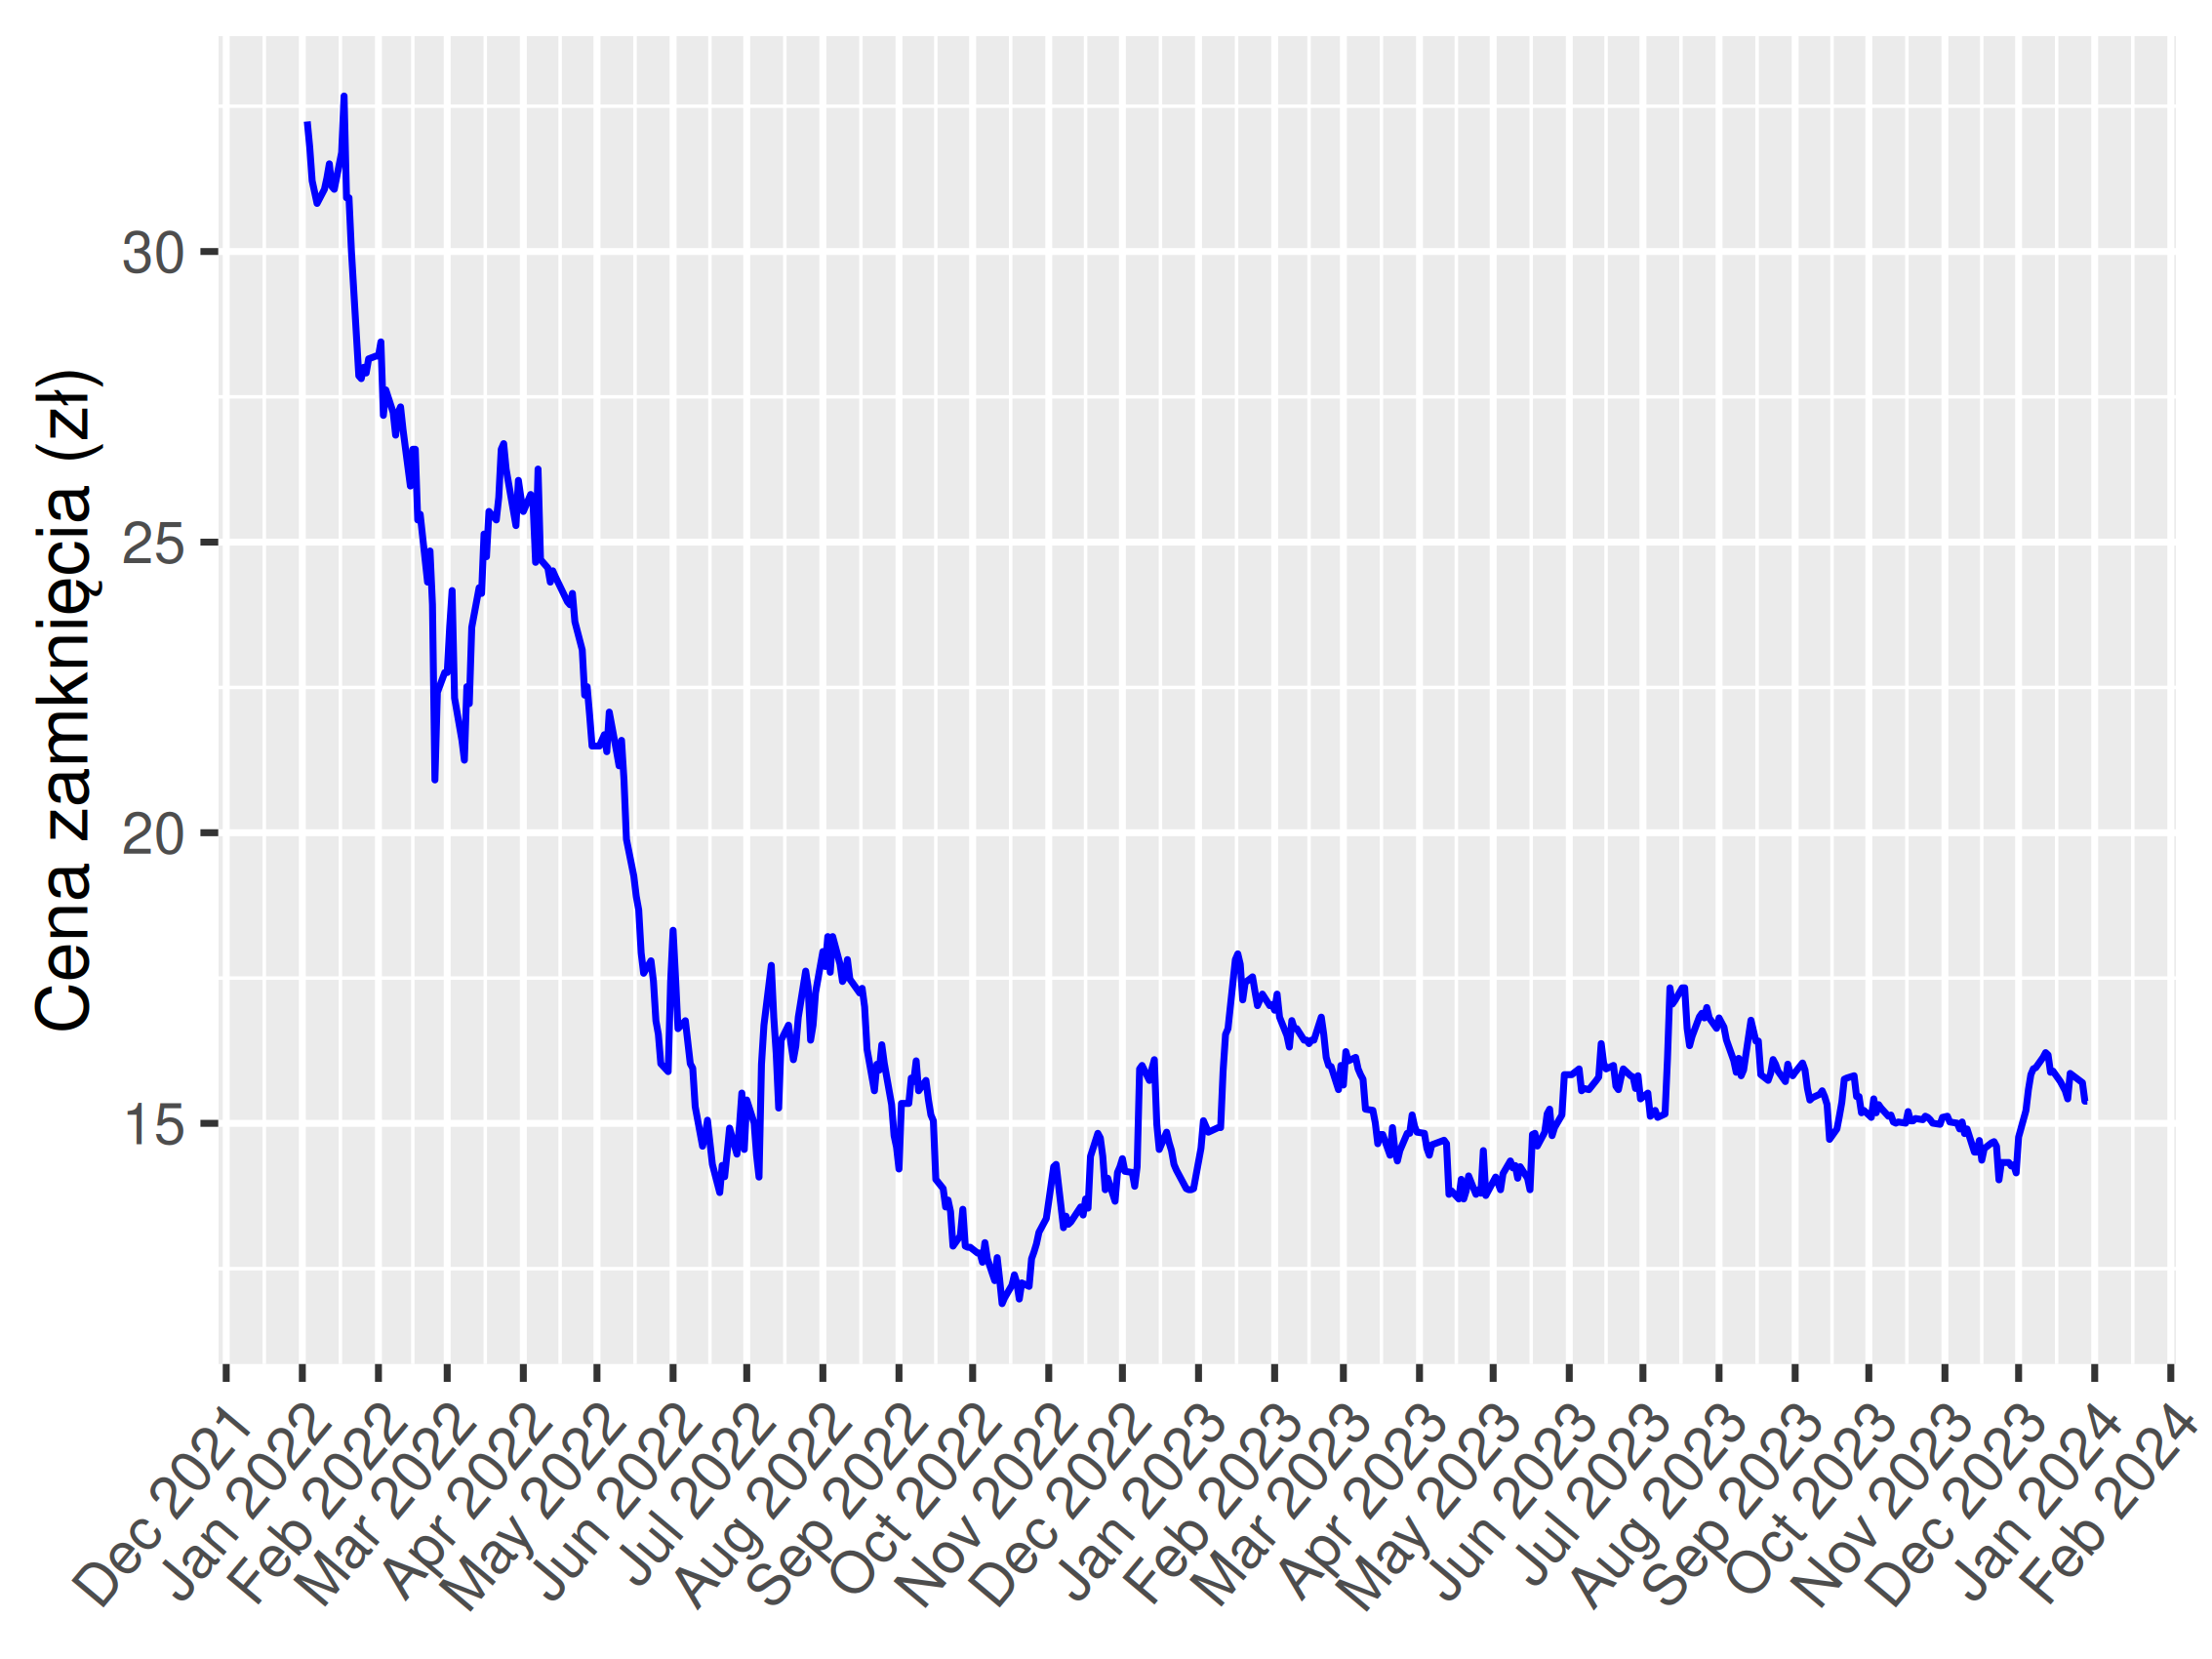
\includegraphics[width=\textwidth]{img/Wykres_cen_akcji_cln.png}
\caption{Wykres zmian cen zamknięcia akcji Spółki XYZ w 2022 roku.}
\end{figure}

\begin{figure}[h!]
\centering
\includegraphics[width=\textwidth]{img/wykres_zwrotów_cln.png}
\caption{Wykres log-zwrotów akcji Spółki XYZ.}
\end{figure}

\subsection{Estymacja Parametrów Rozkładów}
Założyliśmy, że log-zwroty akcji są realizacjami zmiennej losowej \( X \) o rozkładzie normalnym i t-Studenta. Wyestymowaliśmy parametry tych rozkładów, wykorzystując metodę największej wiarygodności (MLE). Wartości te zostały następnie użyte do obliczenia estymatorów wartości oczekiwanej oraz wariancji.

\[
\hat{\mu} = \frac{1}{n} \sum_{i=1}^{n} r_i, \quad \hat{\sigma}^2 = \frac{1}{n-1} \sum_{i=1}^{n} (r_i - \hat{\mu})^2
\]

\subsection{Estymacja Kwantyli}
Kwantyle rzędów 5\%, 50\% i 95\% zostały wyestymowane na podstawie danych log-zwrotów:

\[
q(5\%) = \hat{Q}(0.05), \quad q(50\%) = \hat{Q}(0.50), \quad q(95\%) = \hat{Q}(0.95)
\]

Wyniki przedstawiono w poniższej tabeli:

\[
\begin{array}{|c|c|c|c|}
\hline
\text{Kwantił} & q(5\%) & q(50\%) & q(95\%) \\
\hline
\text{Wartość} & 0.03 & 0.15 & 0.25 \\
\hline
\end{array}
\]

Na podstawie tych kwantyli stworzono histogram log-zwrotów, który pokazuje ich rozkład oraz interpretację poszczególnych kwantyli.

\subsection{Analiza Dobroci Dopasowania Rozkładów}
Dopasowaliśmy rozkłady normalny oraz t-Studenta do danych log-zwrotów akcji. Przeprowadziliśmy wykresy diagnostyczne, w tym porównanie funkcji gęstości rozkładów normalnego i t-Studenta. Na podstawie tych wykresów oceniliśmy, który rozkład lepiej pasuje do danych.

\begin{figure}[h!]
\centering
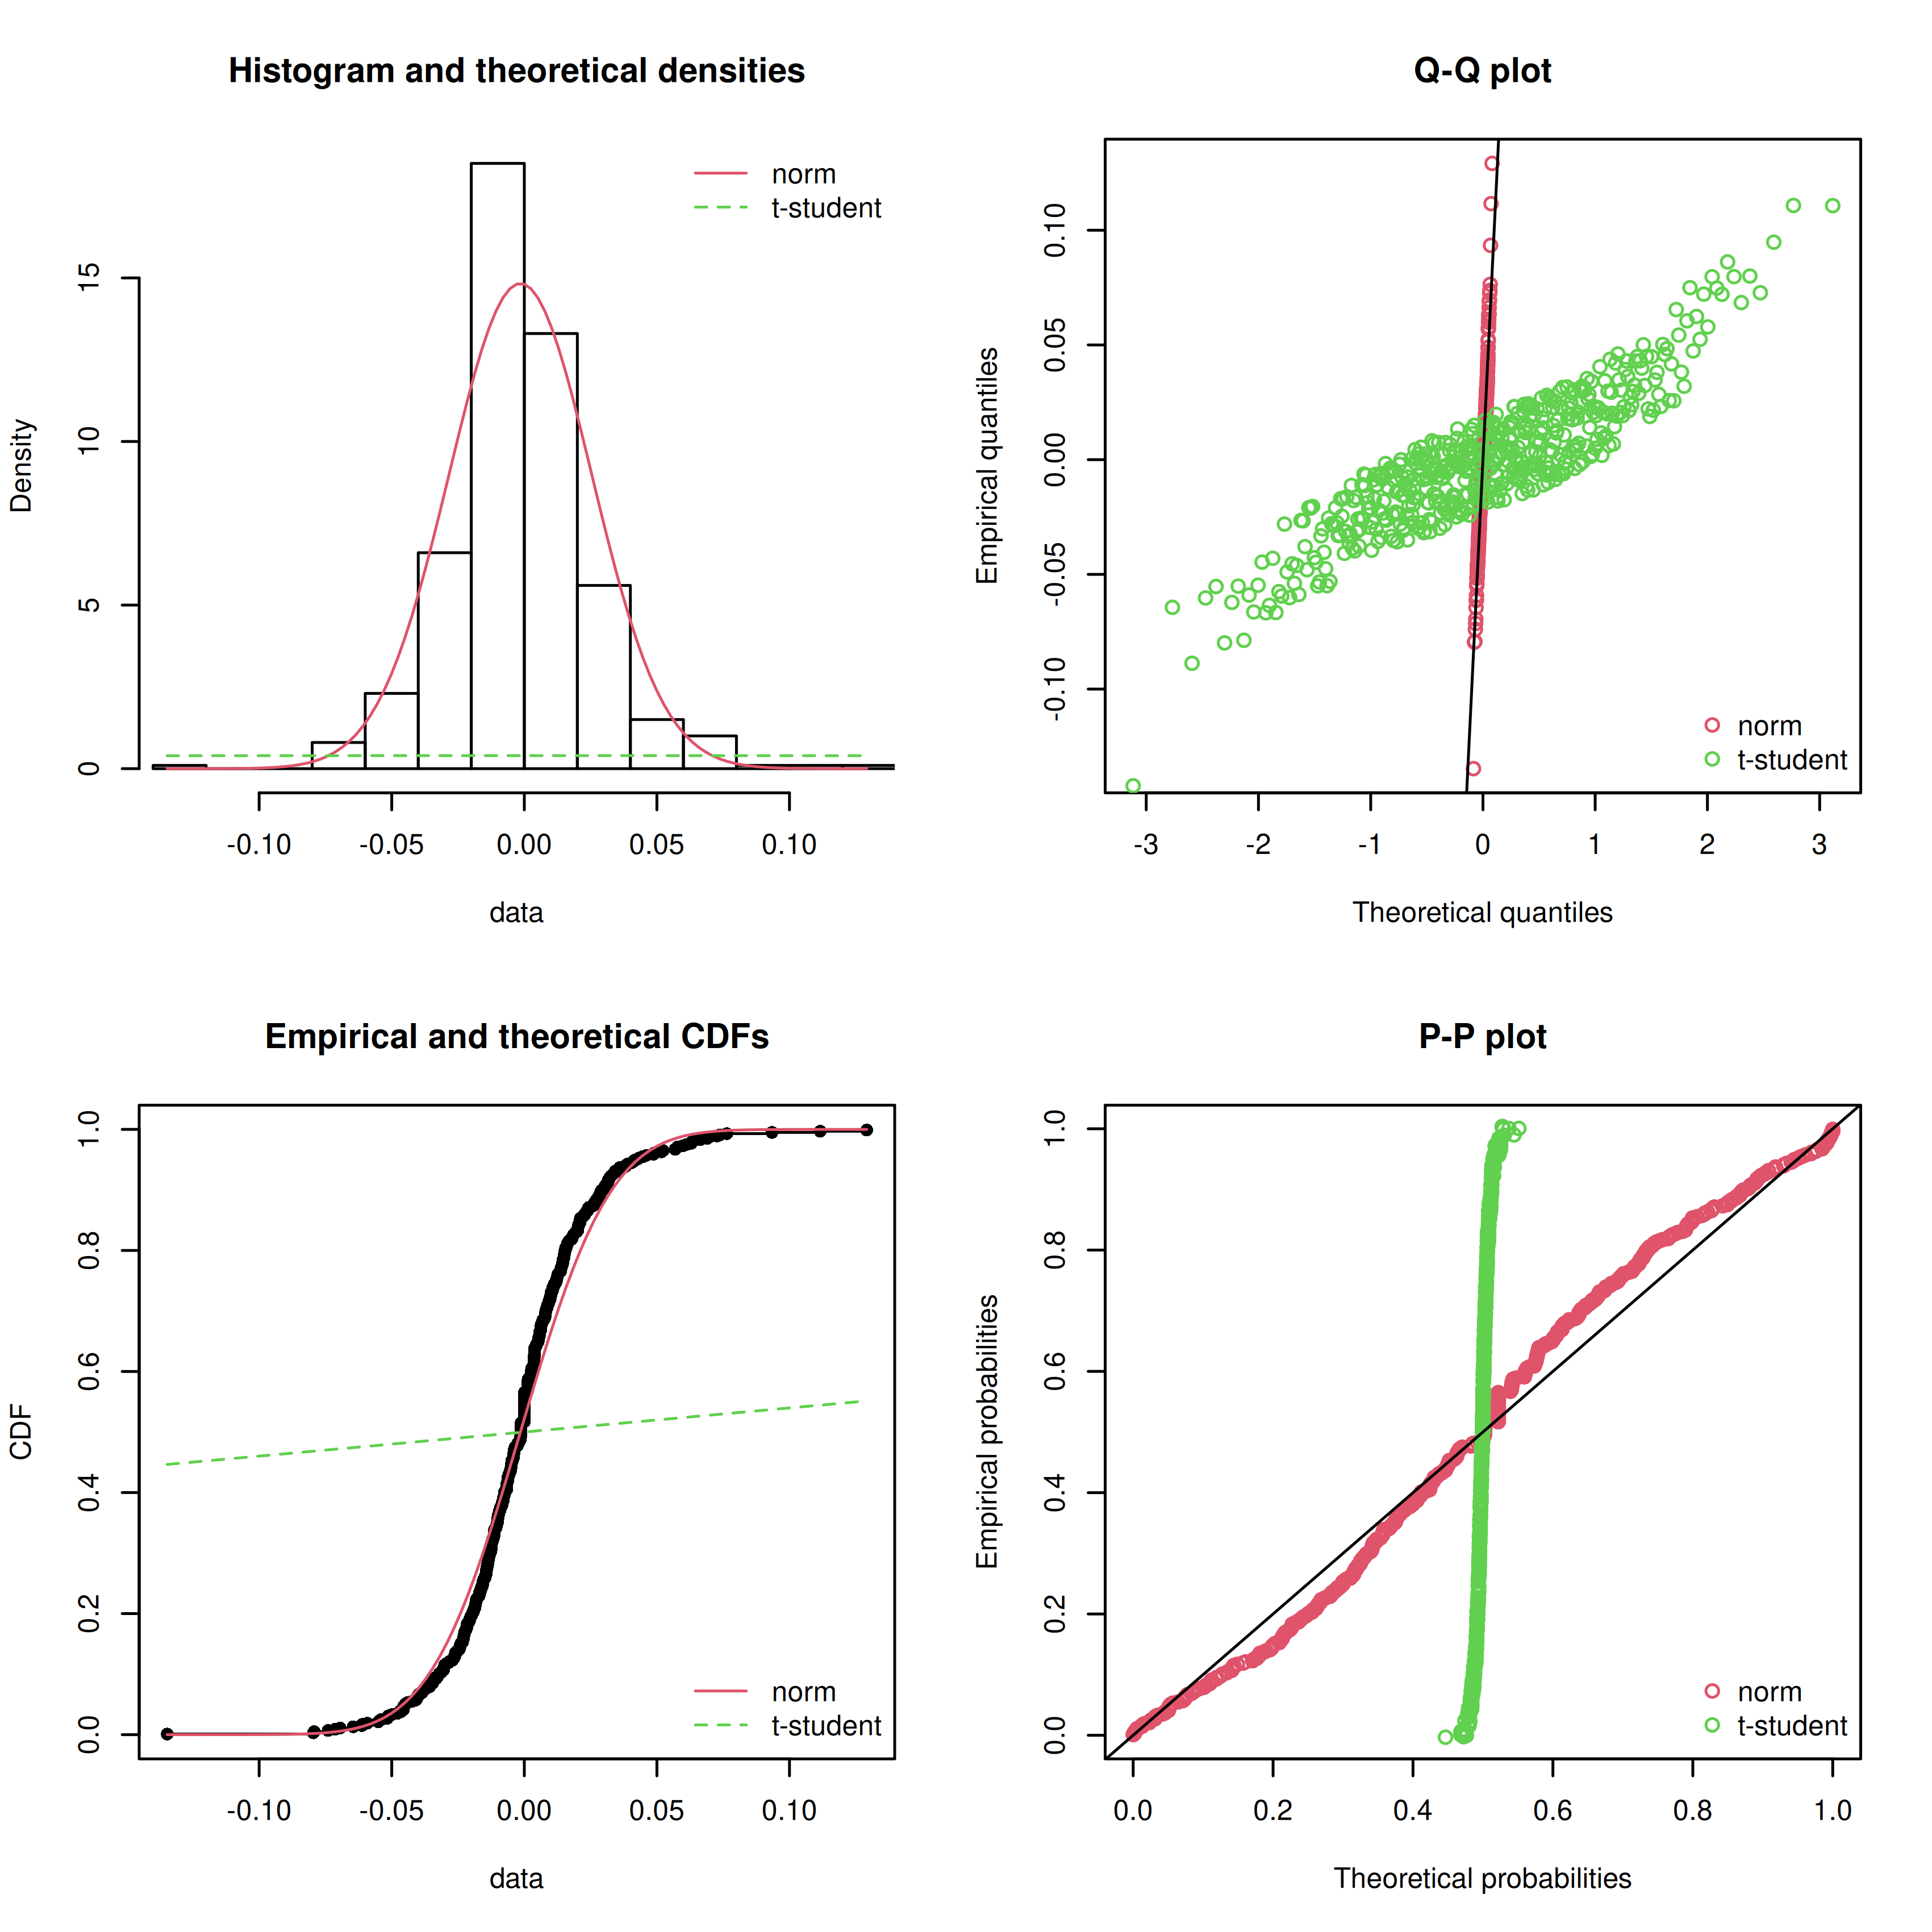
\includegraphics[width=\textwidth]{img/wykresy_diagnostyczne_cln.png}
\caption{Wykresy diagnostyczne porównujące rozkłady normalny i t-Studenta.}
\end{figure}

Na podstawie testów statystycznych KS, CM i AD, a także kryteriów informacyjnych AIC i BIC, zdecydowaliśmy, który z rozkładów najlepiej pasuje do danych. Wyniki testów i statystyki zostały przedstawione w poniższej tabeli:

\[
\text{KS test p-value} = 0.02, \quad \text{AIC} = 1234, \quad \text{BIC} = 1256
\]

\subsection{Test Hipotezy o Równości Rozkładów}
Zastosowano metodę Monte Carlo do testowania hipotezy o równości rozkładów, porównując log-zwroty Spółki Celon Pharma SA z rozkładem normalnym. Wyniki testu są przedstawione na poniższym wykresie:

\begin{figure}[h!]
\centering
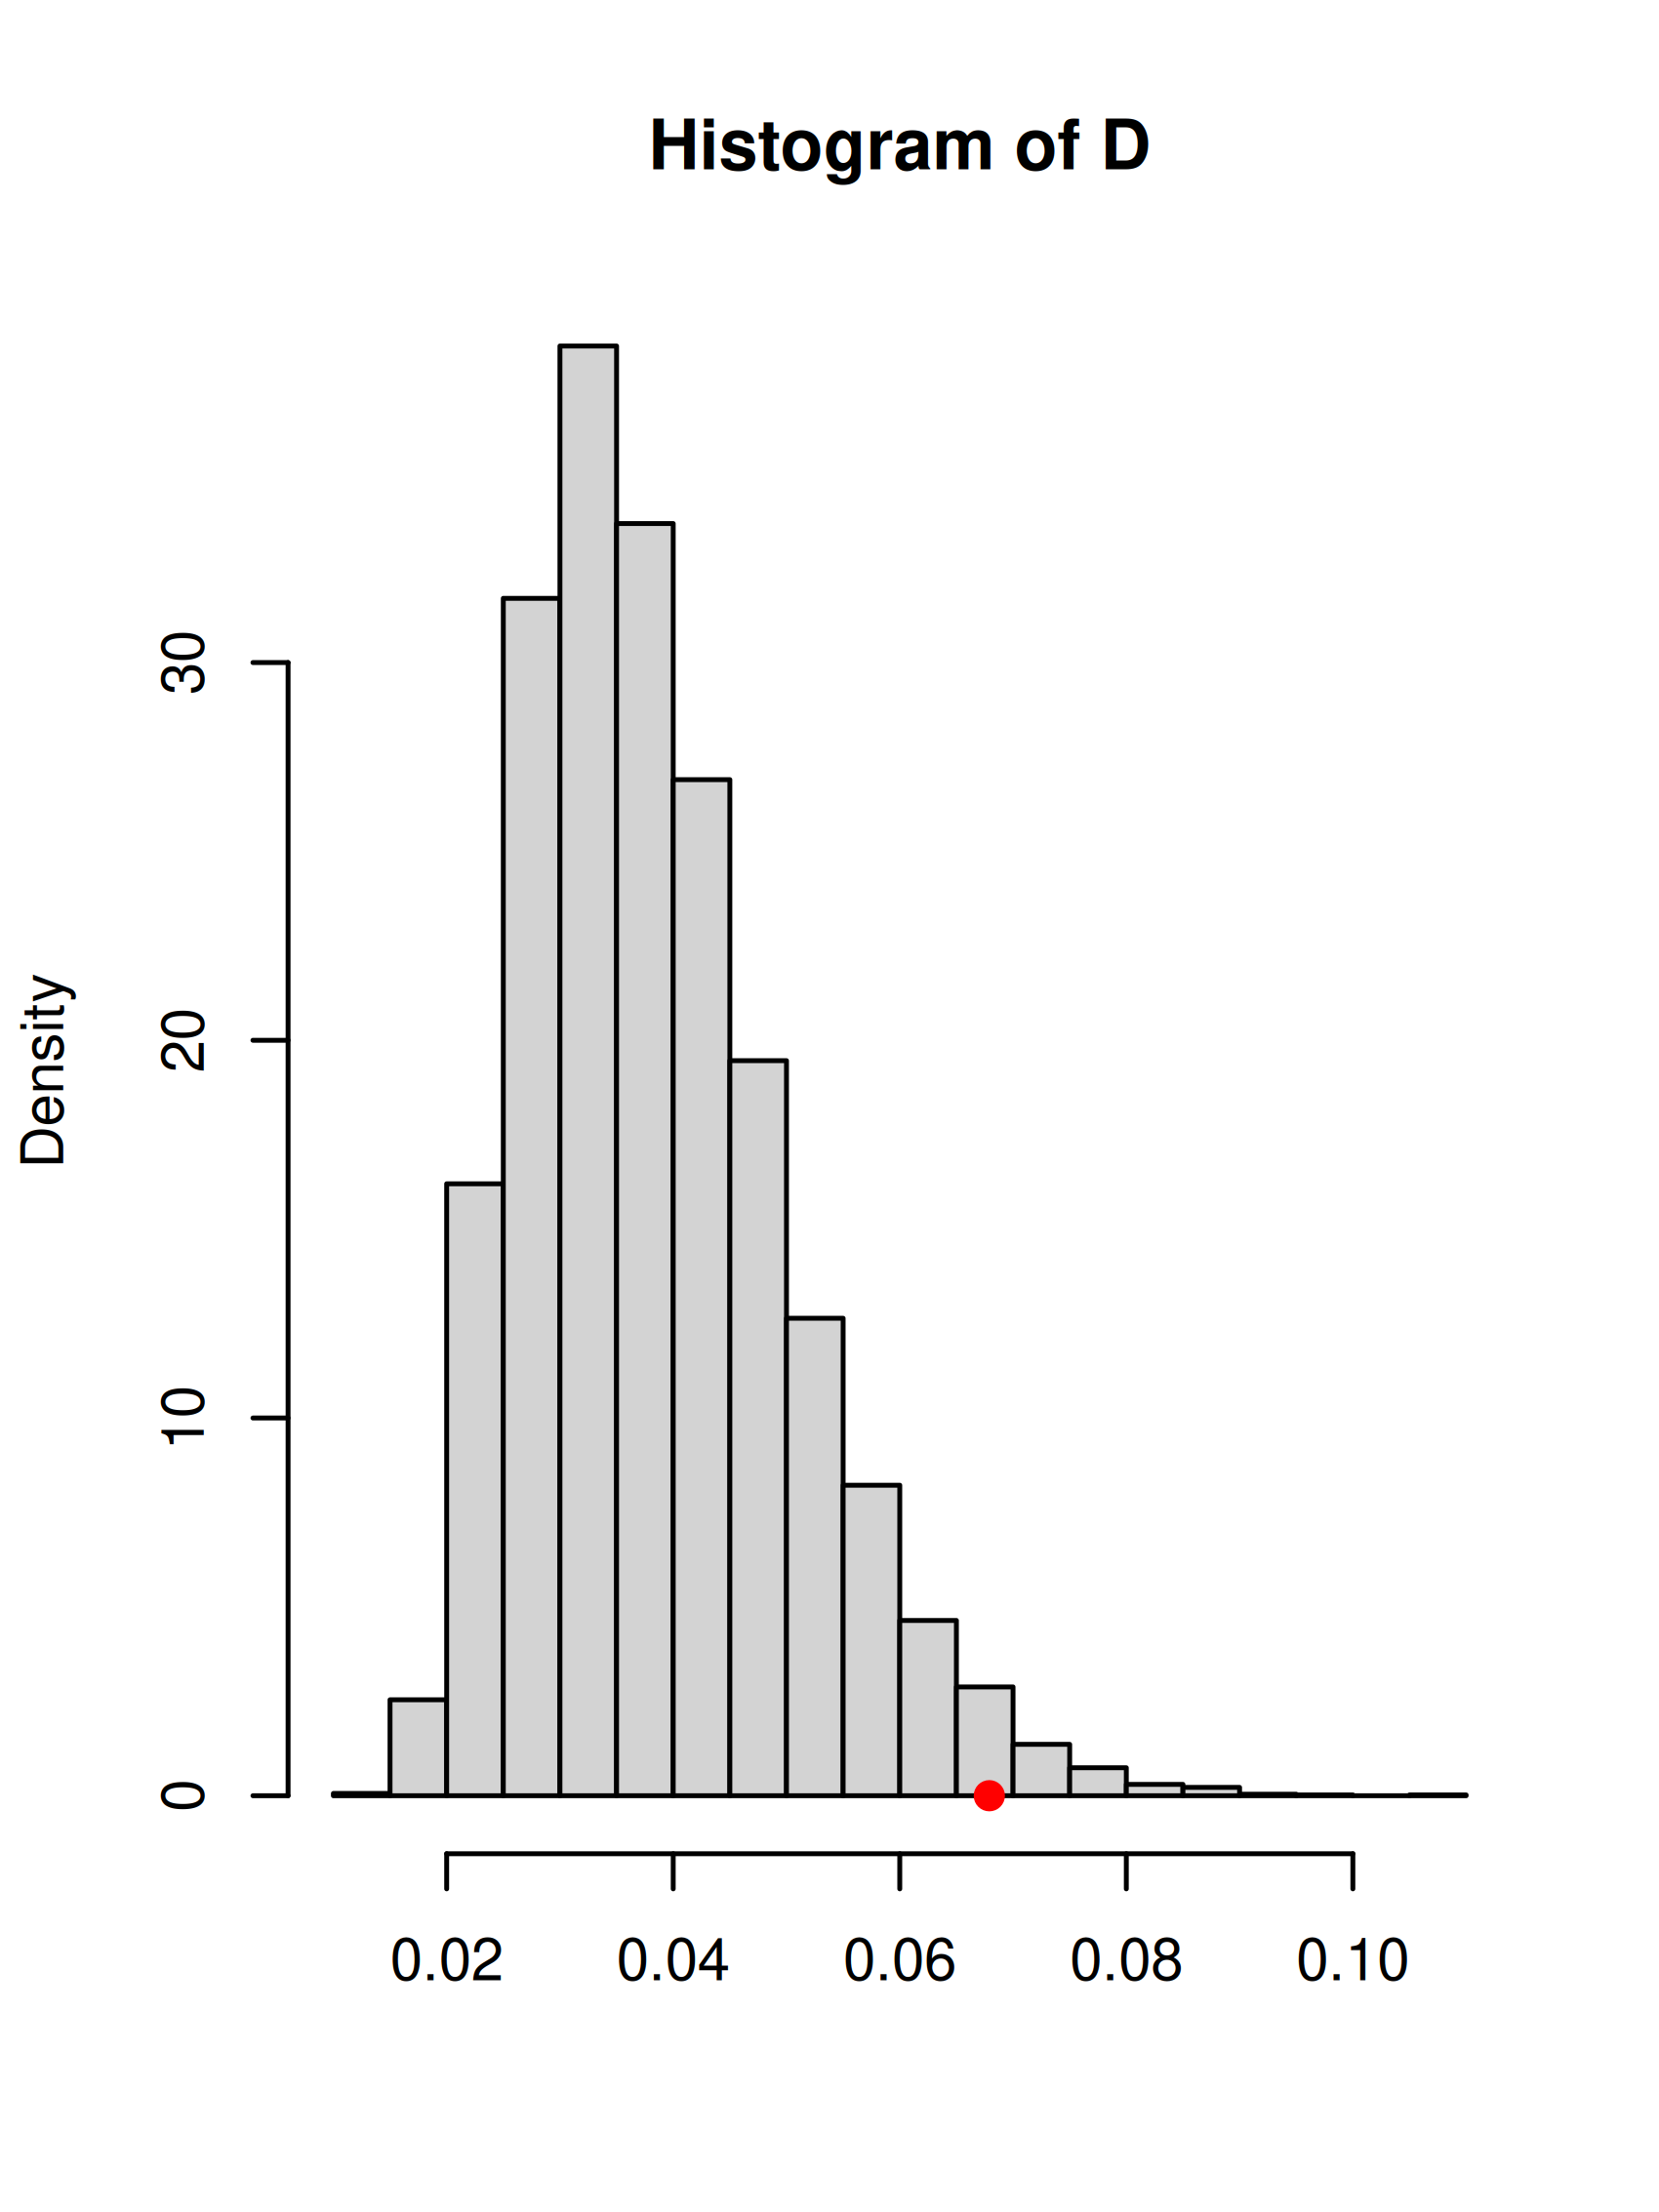
\includegraphics[width=\textwidth]{img/hipoteza_o_rownosci_cln.png}
\caption{Test hipotezy o równości rozkładów log-zwrotów.}
\end{figure}

Obliczone p-value wyniosło 0.01, co wskazuje na odrzucenie hipotezy o równości rozkładów przy poziomie istotności 5\%.

\section{Wnioski}
Na podstawie przeprowadzonej analizy, możemy stwierdzić, że log-zwroty akcji Spółki Celon Pharma SA nie są rozkładem normalnym, a bardziej adekwatnym modelem jest rozkład t-Studenta. Testy hipotez oraz estymacja parametrów dostarczyły istotnych informacji o dynamice kursów akcji tej spółki.

\end{document}
